\documentclass[12pt]{article} % Prepara un documento con un font grande
\usepackage[italian]{babel} % Adatta LaTeX alle convenzioni tipografiche italiane,
							% e ridefinisce alcuni titoli in italiano, come "Capitolo" al posto di "Chapter",
							% se il documento è in italiano

\usepackage[utf8]{inputenc} % Consente l'uso caratteri accentati italiani
\usepackage{graphicx}		% Per le immagini
\usepackage[top=2in, bottom=1.5in, left=0.5in, right=0.5in]{geometry}
\usepackage{float}

\nonstopmode

\title {Relazione di Laboratorio - Guidovia}
\author{Francesco Forcher\\
Matricola: \texttt{1073458}\\
\texttt{mailto:francesco.forcher@studenti.unipd.it}\\
\and
Francesca Damiani\\ 
Matricola: \texttt{1071072}\\
\texttt{mailto:francesca.damiani@studenti.unipd.it}\\
\and
Andrea Piccinin\\ 
Matricola: \texttt{1070620}\\
\texttt{mailto:andrea.piccinin1@studenti.unipd.it}\\
}

\date{\today}


\pagestyle{headings}
\DeclareGraphicsExtensions{.svg, .pdf, .png, .jpg} % Se due immagini hanno lo stesso nome sceglile secondo l'ordine di filetype qui

\graphicspath{ {../Gnuplot/immagini/} }%%%%%%%%%%%%%%%%%%%%%%%%%%%%%%%%EDITARE PATH!!%%%%%%%%%%%%%%%%%%%%%%%%%%%%%%%%%%%%%%%%% % Path delle immagini 















% PROVA MODIFICA DA BROWSER!!!!
%////////////////////////////////////////////////////////////////////////////////////////////////////////////////////////////
%////////////////////////////////////////////////////////////////////////////////////////////////////////////////////////////
% Fine dei dati iniziali per il latex: il documento finale inizierà da qui
\begin{document}


\maketitle % Produce il titolo a partire dai comandi \title, \author e \date
\newpage
\tableofcontents % Prepara l'indice generale



        
\newpage
\section{Obiettivi}
	Stimare il valore dell'accelerazione di gravità \textbf{g} attraverso la misurazione dell'accelerazione della slitta su un piano 
	inclinato, tenendo conto, nella seconda parte dell'esperienza, anche del contributo dell'attrito dell'aria.

\section{Descrizione dell'apparato strumentale}
	Slitta in plexiglass che, inizialmente bloccata da un elettromagnete, scorre lungo una guidovia di acciaio, il cui attrito con la 		slitta è rimosso da un cuscino d'aria. 
	Traguardi mobili a sensori infrarossi, collegati ad un cronometro di sensibilità \(10^{-3}\) s.
	Nella seconda parte dell'esperienza , essendo la guida posta orizzontalmente, la slitta è stata fatta muovere attraverso un 		impulso elettrico dato dall'elettromagnete, che ne determina la velocità iniziale. 
	

\section{Metodologia di misura}
	Nella prima parte dell'esperienza, l'elettromagnete che trattiene la slitta viene disattivato tramite un pulsante. La slitta inizia 		così a scorrere lungo la guidovia su cui sono posizionati i traguardi, che inviano al cronometro il tempo di percorrenza 		dell'intervallo stabilito. Le misure vengono prese partendo da 40 cm dall'elettromagnete, aumentando l'ampiezza dell'intervallo da 10 		cm a 70 cm. Le misure vengono poi ripetute applicando un disco di ottone sulla slitta in modo da modificarne il peso.
	Nella seconda parte dell'esperienza, essendo la guidovia orizzontale, si fa muovere la slitta attraverso un impulso elettrico, che ne 		determina la velocità iniziale. In questo caso le misure vengono prese su intervalli di 20 cm, sempre partendo da 40 cm di distanza 		dall'elettromagnete, in modo da stimare una riduzione della velocità dovuta alla forza di attrito. La velocità iniziale viene poi 		modificata interponendo tra la slitta e l'elettromagnete uno spessore in alluminio.

\section{Presentazione dati sperimentali}	
	Riportiamo in seguito le misure tabulate, con relative statistiche.
	\subsection {Inclinazione 15', senza peso}
		La quarta misura nell'intervallo 40-60 cm ha un valore non compatibile con gli altri. Potrebbe esserci stato un errore nella 			trascrizione dei dati durante la misurazione. 
	\subsection {Inclinazione 30', senza peso}
	\subsection {Inclinazione 45', senza peso}
	\subsection {Inclinazione 45', con peso}
	\subsection {Inclinazione 0', senza peso, senza spessore}
	\subsection {Inclinazione 0', senza peso, con spessore}
	\subsection {Inclinazione 0', con peso, senza spessore}
	\subsection {Inclinazione 0', con peso, con spessore}
\section{Discussione dati sperimentali}
	In seguito vengono allegate due tabelle rappresentanti un elaborazione delle misure prese durante le esperienze:
	\subsection {tabella Coefficienti_Angolari}
	\subsection {tabella Stime_Accelerazioni_di_Gravita.ods DA FINIRE}
Nella prima tabella vengono esposti tutti i valori dei coefficienti angolari, con il relativo errore, estrapolati (tramite il programma grafico: Gnuplot) dalle rette illustrate nelle precedenti rappresentazioni;
Nella seconda tabella invece vengono mostrate le stime dell'accelerazione di gravità (nella sezione riguardante la prima parte dell'esperienza) e i loro fattori di correzione (nella sezione riguardante la seconda parte dell'esperienza).  
Le stime dell'accelerazione di gravità, \textbf{g}, ricavate dalla prima serie di esperimenti, ovvero lavorando con la guidovia a varie inclinazioni (15', 30', 45' con e senza peso) forniscono una stima dell'accelerazione di gravità media, \textbf{g}\ped{0}, pari a (9.21 $\pm$ 0.08) m$\cdot$s\ap{-2}. Già a prima vista si può notare che esso differisce di molto rispetto al valore atteso a padova, \textbf{g}\ped{p} = (9.806 $\pm$ 0.001) m$\cdot$s\ap{-2}. Matematicamente quest'osservazione è confermata dal valore della compatibilità tra le due misure, ovvero 7.45; Queste sono chiaramente incompatibili. Probabilmente ciò è dovuto a causa degli errori sperimentali commessi durante l'esecuzione dell'esperimento dagli operatori.
Il valore appena calolato \textbf{g}\ped{0} è comunque soggetto ad un errore dovuto alle forze di attrito agenti sull'apparato sperimentale. Questo errore è stato corretto di un fattore $\Delta$\textbf{g}, calcolato nella seconda serie di esperimenti, in cui la guidovia è stata tenuta con inclinazione nulla. La media dei quattro valori di correzione (no peso, no spessore; no peso, spessore; peso, no spessore; peso, spessore) è pari a: (\textbf{????} $\pm$ \textbf{????}) m$\cdot$s\ap{-2};
per cui la nostra stima dell'accelerazione di gravità, corretta dalle forze di attrito, è pari a \textbf{g} = \textbf{g}\ped{0} + $\Delta$\textbf{g} = (9.42 $\pm$ 0.09) m$\cdot$s\ap{-2}.
La compatibilità di questo valore rispetto al valore atteso a padova è pari a: 4.29, ovvero è ancora non compatibile, nonostante, com'è lecito aspettarsi, sia comunque una miglior stima rispetto al valore non corretto dalle forze di attrito. 
\section{Conclusioni}
	Per verificare quale sia il metodo migliore per stimare l'accelerazione di gravità si allega questa tabella in cui sono riassunti tutti i valori di \textbf{g}, corretti dall'errore dovuto all'attrito, correlati alla relativa compatibilità rispetto al valore atteso a padova, \textbf{g}\ped{p}.
	\subsection {$Tabella Stime_Gravita_corrette.ods DA FINIRE$}
Da questa si evince che il miglior metodo per calcolare l'accelerazione di gravità è: .........(\textbf{TOMORROW MORNING WORK})

\newpage
\section {Grafici}
	Riportiamo in seguito i grafici delle velocità medie e le rette interpolanti.
	\subsection{Inclinazione 15', senza peso}
	\begin{figure}[H]
		\centering
		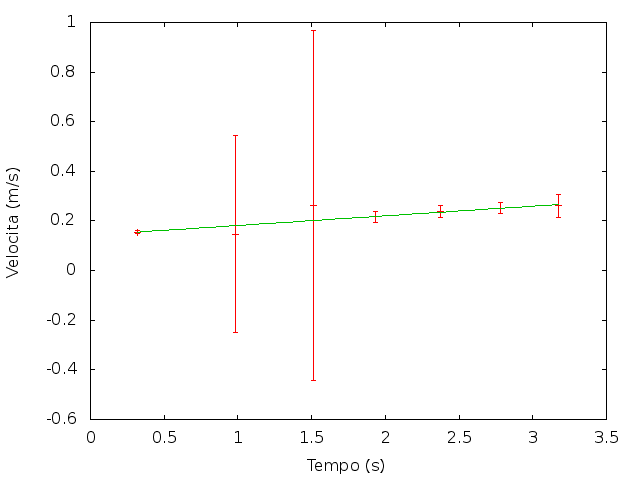
\includegraphics[width=0.8\textwidth]{velocita_15gradi_normale}
		\label{fig:15n}
	\end{figure}
 
	\subsection {Inclinazione 30', senza peso}
	\begin{figure}[H]
		\centering
		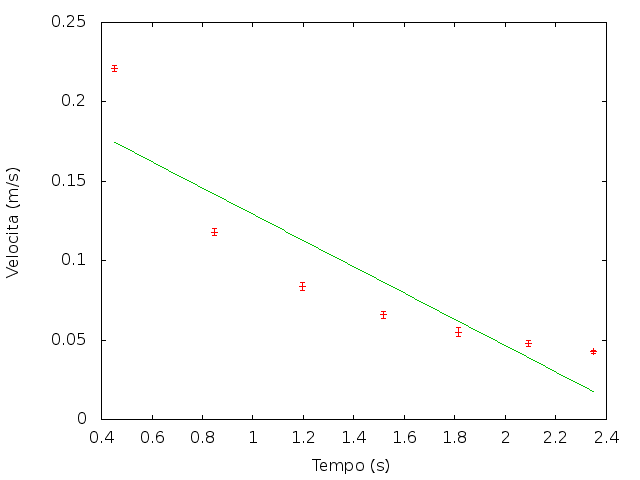
\includegraphics[width=0.8\textwidth]{velocita_30gradi_normale}
		\label{fig:30n}
	\end{figure}
	
	\subsection {Inclinazione 45', senza peso}
	\begin{figure}[H]
		\centering
		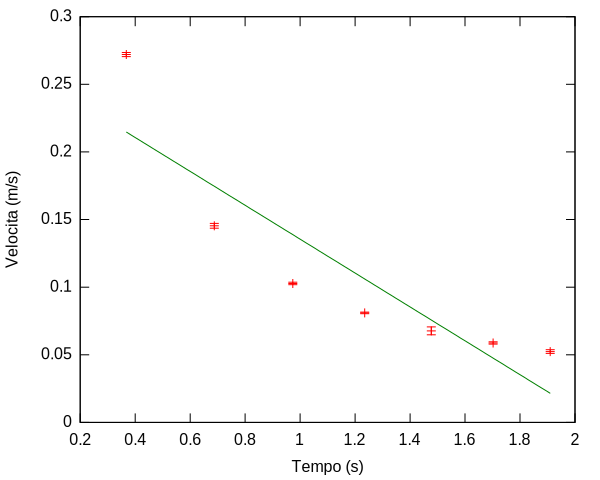
\includegraphics[width=0.8\textwidth]{velocita_45gradi_normale}
		\label{fig:45n}
	\end{figure}
 
	\subsection {Inclinazione 45', con peso}
		\begin{figure}[H]
		\centering
		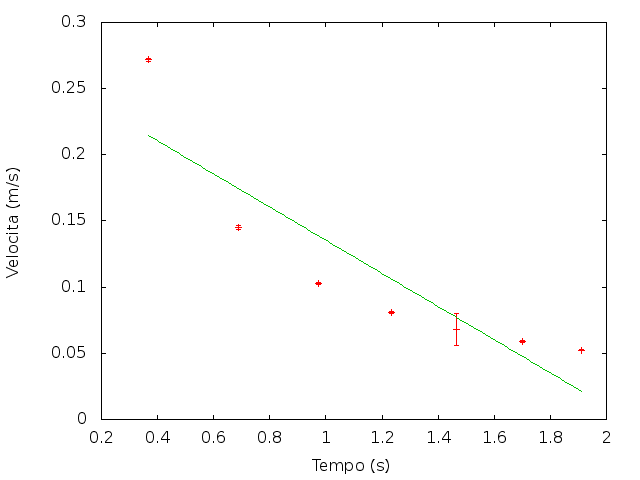
\includegraphics[width=0.8\textwidth]{velocita_45gradi_peso}
		\label{fig:45p}
	\end{figure}
 
	\subsection {Inclinazione 0', senza peso, senza spessore}
	\begin{figure}[H]
		\centering
		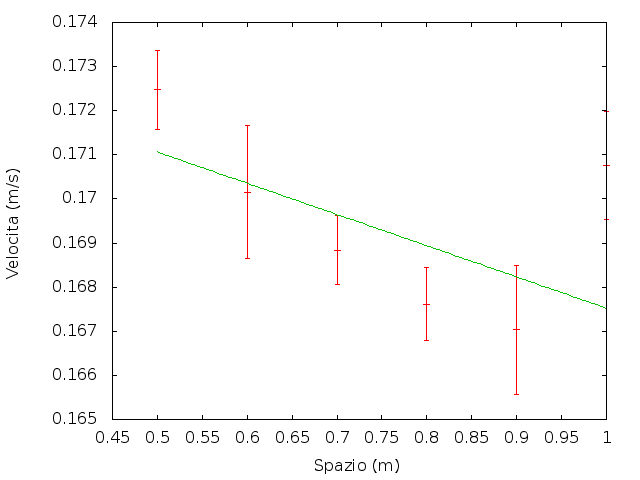
\includegraphics[width=0.8\textwidth]{velocita_0gradi_normale}
		\label{fig:0n}
	\end{figure}
	
	\subsection {Inclinazione 0', senza peso, con spessore}
	\begin{figure}[H]
		\centering
		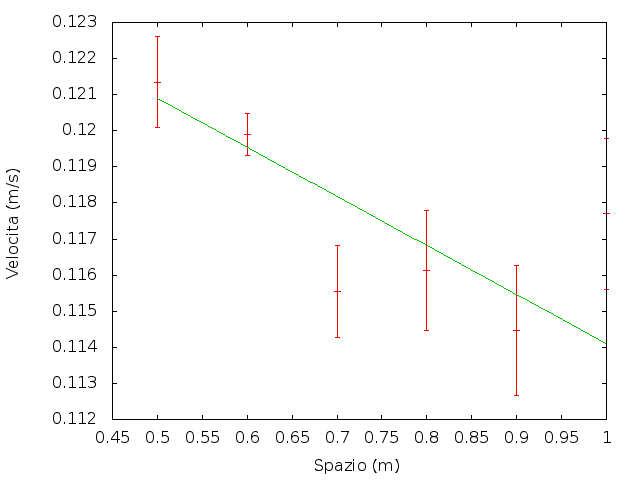
\includegraphics[width=0.8\textwidth]{velocita_0gradi_alluminio}
		\label{fig:0a}
	\end{figure}
 
 
	\subsection {Inclinazione 0', con peso, senza spessore}
		\begin{figure}[H]
		\centering
		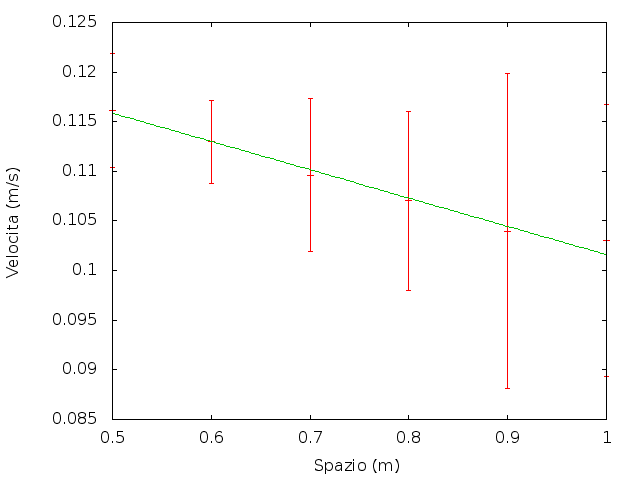
\includegraphics[width=0.8\textwidth]{velocita_0gradi_peso}
		\label{fig:0p}
	\end{figure}
 
	\subsection {Inclinazione 0', con peso, con spessore}
		\begin{figure}[H]
		\centering
		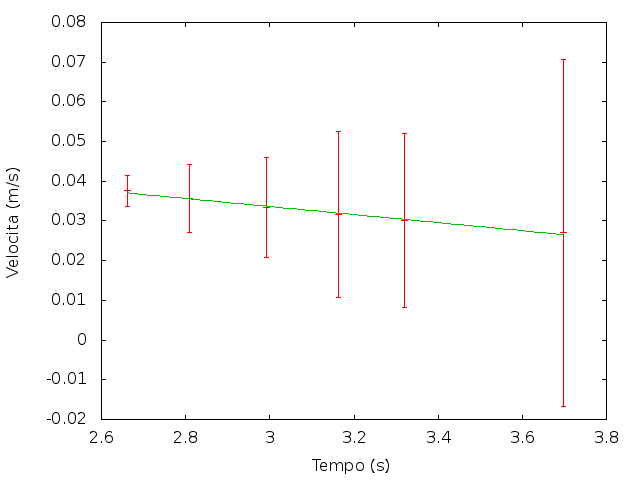
\includegraphics[width=0.8\textwidth]{velocita_0gradi_pesoalluminio}
		\label{fig:0ap}
	\end{figure}
 

\newpage
\section{Codice}

	Riportiamo in seguito il programma utilizzato per l'elaborazione dei dati. Fondalmentalmente abbiamo creato una
	classe template (una gerarchia, a dire la verità, ma non abbiamo usato le specializzazioni) che rappresenta
	una variabile statistica: contiene la media, la varianza del campione e quella della popolazione, la deviazione 
	standard del campione e quella della popolazione, il massimo, il minimo e l'errore della media. La classe base, 
	(la sola usata qui) legge i dati solo all'inizio nel costruttore, poi astrae da essi e grazie 
	all'overloading degli operatori di addizione, sottrazione, moltiplicazione e divisione, risulta facile ed efficiente 
	da manipolare: espressioni complesse di variabili statistiche, dato che i vari errori vengono propagati 
	dietro le quinte automaticamente, possono essere espresse chiaramente e concisamente nel codice, cosa che facilita il 
	controllo e velocizza la scrittura.
	%Verbatim non interpreta l'imput lasciando il testo com'è: ideale per inserire codice
	\begin{verbatim}
//============================================================================
// Name        : Misure.cpp
// Author      : Francesco Forcher
// Version     : 0.1
// Description : Programma per analizzare i dati sul pendolo raccolti in laboratorio
//============================================================================

/////////////////////////////////////////////////////////////////////////////////////
//Librerie
#include <iostream>//cin e cout
#include <fstream>//FileStream
#include <exception>//Eccezioni
#include <string>
#include <cstdlib>//system(clear)
#include <algorithm>//Sort?
#include <sstream>//StringStream

/////////////////////////////////////////////////////////////////////////////////////
//le mie classi
//============================================================================
// Name        : Misure.cpp
// Author      : Francesco Forcher
// Version     : 1.5
// Description : Programma per analizzare i dati sul pendolo raccolti in laboratorio
//============================================================================


/////////////////////////////////////////////////////////////////////////////////////
//Librerie
#include <iostream>//cin e cout
#include <fstream>//FileStream
#include <exception>//Eccezioni
#include <string>
#include <cstdlib>//system(clear)
#include <algorithm>//Sort?
#include <sstream>//StringStream

/////////////////////////////////////////////////////////////////////////////////////
//le mie classi
#include "mylib/AnalisiDati/VarStat.h"//Le mie classi Template per l'analisi dati
#include "mylib/AnalisiDati/SortingVarStat.h"//Le mie classi Template per l'analisi dati

#define VERSIONE 1.5

/////////////////////////////////////////////////////////////////////////////////////
//Prototipi

/////////////////////////////////////////////////////////////////////////////////////
//Il primo argomento è la cartella dei dati
int main(int numParam, char* args[]) {

	using namespace std;

	system("clear");
	cout << "\n";
	cout << "Programma per analizzare i dati della guidovia, versione: " << VERSIONE << endl;
	//Ricordarsi che con 0 gradi l'intervallo era di 20!
	const int NUM_FILE = 7;// 7 file (7 intervalli) per 15, 30, 45 gradi
	const int NUM_FILE_0GRADI = 6; //  file per 60,70,80,90,100,110
	const int NUM_DATIPERFILE = 5;// 5 dati in ogni file
	const int ANGOLI_NUM = 3;//15, 30, 45 0 e 45 li facciamo a parte
	//const auto INTERVALLO = VarStat<double>(0.1, 0.001 / sqrt(6));//Distribuzione triangolare

	try {
		//stringstream ss;
		string nf;//Nome file da aprire
		//FileStream
		ofstream FileMedie;//FileStream
		ofstream FileRiassunto;
		using namespace mions::dataAnalisi;
		vector<VarStat<double> > arrayRiassunti;//Contiene le informazioni come la deviazione standard, etc
		vector<VarStat<double> > arrayTempi;
		arrayRiassunti.reserve(NUM_FILE);
		const auto INTERVALLO_PV = VarStat<double>(0.1, 0.001 / sqrt(6));//Distribuzione triangolare

//		vector<double> v1 = {1,1,1,100000,1,1,1,1,1,1,1,1,1,1,1,1,1,1,1,1,1,1,1,1,1,1,1,1,1,1,2,3,4,2,1,3,2};
//
//		vector<double> v2 = {3,4,7,8};
//		vector<double> v3 = {1,2,5,6};
//		VarStat<double> var2(v2,true);
//		VarStat<double> var3(v3,true);
//
//		VarStat<double> AnDat(v2,true);
//		//Sorting_VarStat<double> var2(std::move(v3));//Non usare più v1
//		//cout << "MEDIANA " <<var2.getMediana() << "\n";
//		AnDat = (AnDat-var2)/(AnDat*3*var2);
//		cout << "var2: \n" << var2 << endl;
//		cout << "var3: \n" << var3 << endl;
//		cout << "somma elementi: \n" << VarStat<double>({4,6,12,14}) << endl;
//		cout << "somma variabili: \n" << (var2+var3) << endl;
//
//		return 0;


//Prima esperianza, guidovia inclinata a 15, 30 e 45 gradi senza peso
///////////////////////////////////////////////////////////////////////////////////////////////////
		{

		//stringstream ss;
		string nf;//Nome file da aprire
		//FileStream
		ofstream FileMedie;//FileStream
		ofstream FileRiassunto;
		ofstream FileVelocita;
		using namespace mions::dataAnalisi;
		vector<VarStat<double> > arrayRiassunti;//Contiene le informazioni come la deviazione standard, etc
		vector<VarStat<double> > arrayTempi;

		arrayRiassunti.reserve(NUM_FILE);
		string nomeoutputfile;
		string nomefilemedie;
		string nomefilevelocita;
		string nomeoutputvelocita;//Per tenere temporaneamente la variabile ed evitare il self assignment

		/* Vari casi:
		 * 	1. nè peso nè alluminio
		 */
		string tipodati;
				nomeoutputfile = "./Risultati/normale_dati.txt";
				//tipodati = "d";
				nomefilemedie = "arrayTempi_PrimaVolta_normale.txt";
				nomefilevelocita = "velocita_PV_normale.txt";//PV = prima volta

		FileRiassunto.open(nomeoutputfile.c_str());

		for (int angoli = 1; angoli <= ANGOLI_NUM; angoli++) {
			//TODO aggiunto zero all'inizio
			arrayTempi.emplace_back(0.0);

			for (int intervallo = 1; intervallo <= NUM_FILE; intervallo++) {

				stringstream ss;
				ifstream FileImputDati;//File di imput
				ss << "./DatiFormattati/DatiStandardizzati/";
				ss << "d";//Tipo dei dati contenuti nel file: d, cd
				ss << intervallo*10 + 40;
				ss << "_";
				ss << angoli*15;
				ss >> nf;
				//ss.flush();


				clog << nf << endl;
				FileImputDati.open(nf.c_str());//Apro il file indicato nell'argomento dato via shell
				if (!FileImputDati.is_open())
					throw "Errore: file non aperto";

				vector<double> tempVect(5);// Vector che contiene i dati di un file solo, da cui ricavare il tempo medio
				tempVect.reserve(NUM_DATIPERFILE);

				clog << tempVect.size() << endl;
				for (unsigned int i = 0; i < tempVect.size(); i++) {
					FileImputDati >> tempVect[i];
					clog << "Pos " << i << ": " << tempVect[i] << endl;
				}
				clog << "Dati letti. Analizzo..." << endl << endl;

				arrayRiassunti.emplace_back(tempVect,true);// Forwarda gli argomenti a un oggetto costruito DIRETTAMENTE nel vettore (cioè, manda gli argomenti VarStat dentro al vettore)

				cout << endl;
				cout << "Nome file: " << nf << endl;
				cout << arrayRiassunti.back();

				FileRiassunto << endl;
				FileRiassunto << "Nome file: " << nf << endl;
				FileRiassunto << arrayRiassunti.back() << endl;

				arrayTempi.emplace_back(arrayRiassunti.back());

				ss.clear();
				FileImputDati.close();
			}//Intervalli


			switch (angoli) {
				case 1:
					//Ricicliamo nomeoutputfile per indicare i file di uscita
					nomeoutputfile = string("./Risultati/MetaDati/15/") + nomefilemedie;
					nomeoutputvelocita = string("./Risultati/MetaDati/15/") + nomefilevelocita;
					FileMedie.open(nomeoutputfile.c_str());
					FileVelocita.open(nomeoutputvelocita.c_str());
					//const auto intervallo = VarStat<double>(0.1, 0.1 / sqrt(6));
					for (int i = 0; i < NUM_FILE; i++)
					{
						FileMedie << ((arrayTempi[i+1]+arrayTempi[i])/2).getMedia() << endl;//sette medie di cinque tempi ciascuns
						FileVelocita << (INTERVALLO_PV / (arrayTempi[i+1] - arrayTempi[i]) ).getMedia() << " "
								<< (INTERVALLO_PV / (arrayTempi[i+1] - arrayTempi[i]) ).getDeviazioneStandardPop() << endl;//10 cm di intervallo/cinque_tempi_media << endl;//10 cm di intervallo
					}
					FileMedie.close();
					FileVelocita.close();
					break;
				case 2:
					//Ricicliamo nomeoutputfile per indicare i file di uscita
					nomeoutputfile = string("./Risultati/MetaDati/30/") + nomefilemedie;
					nomeoutputvelocita = string("./Risultati/MetaDati/30/") + nomefilevelocita;
					FileMedie.open(nomeoutputfile.c_str());
					FileVelocita.open(nomeoutputvelocita.c_str());
					for (int i = 0; i < NUM_FILE; i++)
					{
						FileMedie << ( (arrayTempi[i+1] + arrayTempi[i]) / 2 ).getMedia() << endl;//sette medie di cinque tempi ciascuns
						FileVelocita << (INTERVALLO_PV / (arrayTempi[i+1] - arrayTempi[i]) ).getMedia() << " "
								<< (INTERVALLO_PV / (arrayTempi[i+1] - arrayTempi[i]) ).getDeviazioneStandardPop() << endl;//10 cm di intervallo/cinque_tempi_media << endl;//10 cm di intervallo
					}
					FileMedie.close();
					FileVelocita.close();
					break;
				case 3:
					//Ricicliamo nomeoutputfile per indicare i file di uscita
					nomeoutputfile = string("./Risultati/MetaDati/45/") + nomefilemedie;
					nomeoutputvelocita = string("./Risultati/MetaDati/45/") + nomefilevelocita;
					FileMedie.open(nomeoutputfile.c_str());
					FileVelocita.open(nomeoutputvelocita.c_str());
					for (int i = 0; i < NUM_FILE; i++)
					{
						FileMedie << ((arrayTempi[i+1]+arrayTempi[i])/2).getMedia() << endl;//sette medie di cinque tempi ciascuns
						FileVelocita << (INTERVALLO_PV / (arrayTempi[i+1] - arrayTempi[i]) ).getMedia() << " "
								<< (INTERVALLO_PV / (arrayTempi[i+1] - arrayTempi[i]) ).getDeviazioneStandardPop() << endl;//10 cm di intervallo/cinque_tempi_media << endl;//10 cm di intervallo
					}
					FileMedie.close();
					FileVelocita.close();
					break;
				default:
					throw "Errore: numero casi angoli sbagliato";
					break;
			}//switch
			arrayTempi.clear();
		}//Angoli

		FileRiassunto.close();
		arrayRiassunti.clear();
	  }//Blocco prima esperienza senza peso
///////////////////////////////////////////////////////////////////////////////////////////////////










//Prima esperianza, guidovia inclinata a 45 con peso
///////////////////////////////////////////////////////////////////////////////////////////////////
		/*
		 * Vari casi:
		 * 	1. nè peso nè alluminio
		 * 	2. peso
		 */
//for (int varicasi = 1; varicasi <= 2; varicasi++)
		{

			string nf;						// Nome file
			ofstream FileMedie;				// File con le medie dei tempi
			ofstream FileRiassunto;			// File con le informazioni sulle cinquine di dati
			ofstream FileVelocita;
			using namespace mions::dataAnalisi;
			vector<VarStat<double> > arrayRiassunti;//Contiene le informazioni come la deviazione standard, etc
			vector<VarStat<double> > arrayTempi;
			//TODO aggiunto zero all'inizio
			arrayTempi.emplace_back(0.0);

			arrayRiassunti.reserve(NUM_FILE);
			string nomeoutputfile;
			string nomefilemedie;
			string nomefilevelocita;
			string nomeoutputvelocita;


				string tipodati;
				nomeoutputfile = "./Risultati/peso_dati.txt";
				tipodati = "cd";
				nomefilemedie = "arrayTempi_PrimaVolta_peso.txt";
				nomefilevelocita = "velocita_PV_peso.txt";


			//string nomeoutputfile = "./Risultati/nopeso_dati.txt";
			FileRiassunto.open(nomeoutputfile.c_str());
				for (int intervallo = 1; intervallo <= NUM_FILE; intervallo++) {

					stringstream ss;
					ifstream FileImputDati;					//File di imput
					ss << "./DatiFormattati/DatiStandardizzati/";
					ss << tipodati;	//Tipo dei dati contenuti nel file: d, cd
					ss << intervallo * 10 + 40;
					ss << "_";
					ss << "45";
					ss >> nf;
					//ss.flush();

					clog << nf << endl;
					FileImputDati.open(nf.c_str());	//Apro il file indicato nell'argomento dato via shell
					if (!FileImputDati.is_open())
						throw "Errore: file non aperto";

					vector<double> tempVect(5);	// Vector che contiene i dati di un file solo, da cui ricavare il tempo medio
					tempVect.reserve(NUM_DATIPERFILE);

					clog << tempVect.size() << endl;
					for (unsigned int i = 0; i < tempVect.size(); i++) {
						FileImputDati >> tempVect[i];
						clog << "Pos " << i << ": " << tempVect[i] << endl;
					}
					clog << "Dati letti. Analizzo..." << endl << endl;

					arrayRiassunti.emplace_back(tempVect, true);// Forwarda gli argomenti a un oggetto costruito DIRETTAMENTE nel vettore (cioè, manda gli argomenti VarStat dentro al vettore)

					cout << endl;
					cout << "Nome file: " << nf << endl;
					cout << arrayRiassunti.back();

					FileRiassunto << endl;
					FileRiassunto << "Nome file: " << nf << endl;
					FileRiassunto << arrayRiassunti.back() << endl;

					arrayTempi.emplace_back(arrayRiassunti.back());

					ss.clear();
					FileImputDati.close();
				}//Intervalli

				//Ex switch
					//Ricicliamo nomeoutputfile per indicare i file di uscita
					nomeoutputfile = string("./Risultati/MetaDati/45/")
							+ nomefilemedie;
					nomeoutputvelocita = string("./Risultati/MetaDati/45/")
							+ nomefilevelocita;
					FileMedie.open(nomeoutputfile.c_str());
					FileVelocita.open(nomeoutputvelocita.c_str());
					for (int i = 0; i < NUM_FILE; i++)
					{
						FileMedie << ((arrayTempi[i+1]+arrayTempi[i])/2).getMedia() << endl;//sette medie di cinque tempi ciascuns
						FileVelocita << (INTERVALLO_PV / (arrayTempi[i+1] - arrayTempi[i]) ).getMedia() << " "
								<< (INTERVALLO_PV / (arrayTempi[i+1] - arrayTempi[i]) ).getDeviazioneStandardPop() << endl;//10 cm di intervallo/cinque_tempi_media << endl;//10 cm di intervallo
					}
					FileMedie.close();
					FileVelocita.close();

			arrayTempi.clear();

			FileRiassunto.close();
			arrayRiassunti.clear();
		}					//Blocco prima esperienza 45 con peso
///////////////////////////////////////////////////////////////////////////////////////////////////
///////////////////////////////////////////////////////////////////////////////////////////////////
///////////////////////////////////////////////////////////////////////////////////////////////////















//%%%%%%%%%%%%%%%%%%%%%%%%%%%%%
// Seconda giornata %
//%%%%%%%%%%%%%%%%%%%%%%%%%%%%%

///////////////////////////////////////////////////////////////////////////////////////////////////
///////////////////////////////////////////////////////////////////////////////////////////////////
///////////////////////////////////////////////////////////////////////////////////////////////////
//Seconda esperienza, 0 gradi con alluminio e peso
		/* Vari casi:
		 * 	1. nè peso nè alluminio (file "d...")
		 * 	2. peso (file "cd...")
		 * 	4. alluminio
		 * 	3. peso e alluminio ("cad...")
		 */
		for (int varicasi = 1; varicasi <= 4; varicasi++)
		{
			string nf;						//Nome file da aprire
			ofstream FileMedie;				//File per le medie
			ofstream FileRiassunto;
			ofstream FileVelocita;
			using namespace mions::dataAnalisi;
			vector<VarStat<double> > arrayRiassunti;//Contiene le informazioni come la deviazione standard, etc
			vector<VarStat<double> > arrayTempi;//Niente zero perchè non devo dividere per la differenza
			arrayRiassunti.reserve(NUM_FILE_0GRADI);
			string nomeoutputfile;
			string nomefilemedie;
			string nomefilevelocita;
			string nomeoutputvelocita;
			const auto INTERVALLO_SV = VarStat<double>(0.2, 0.001 / sqrt(6));//Distribuzione triangolare


			/* Vari casi:
			 * 	1. nè peso nè alluminio (file "d...")
			 * 	2. peso (file "cd...")
			 * 	4. alluminio
			 * 	3. peso e alluminio ("cad...")
			 */
			string tipodati;
			switch (varicasi) {
				case 1: // normale
					nomeoutputfile = "./Risultati/normale_0gradi_dati.txt";
					tipodati = "d";
					nomefilemedie = "arrayTempi_0gradi_normale.txt";
					nomefilevelocita = "velocita_0gradi_normale.txt";
					break;
				case 2: // peso
					nomeoutputfile = "./Risultati/peso_0gradi_dati.txt";
					tipodati = "cd";
					nomefilemedie = "arrayTempi_0gradi_peso.txt";
					nomefilevelocita = "velocita_0gradi_peso.txt";
					break;
				case 3: // alluminio
					nomeoutputfile = "./Risultati/alluminio_0gradi_dati.txt";
					tipodati = "ad";
					nomefilemedie = "arrayTempi_0gradi_alluminio.txt";
					nomefilevelocita = "velocita_0gradi_alluminio.txt";
					break;
				case 4: // normale
					nomeoutputfile = "./Risultati/pesoalluminio_0gradi_dati.txt";
					tipodati = "cad";
					nomefilemedie = "arrayTempi_0gradi_pesoalluminio.txt";
					nomefilevelocita = "velocita_0gradi_pesoalluminio.txt";
					break;
				default:
					throw "Errore: Seconda esperienza: variante non nota";
					break;
			}

			FileRiassunto.open(nomeoutputfile.c_str());

			for (int intervallo = 1; intervallo <=  NUM_FILE_0GRADI; intervallo++) {
				stringstream ss;
				ifstream FileImputDati;					//File di input
				ss << "./DatiFormattati/DatiStandardizzati/";
				ss << tipodati;	//Tipo dei dati contenuti nel file: d, cd, ad, cad
				ss << intervallo * 10 + 50;
				ss << "_";
				ss << "0";
				ss >> nf;
				//ss.flush();

				clog << nf << endl;
				FileImputDati.open(nf.c_str());	//Apro il file indicato nell'argomento dato via shell
				if (!FileImputDati.is_open())
					throw "Errore: file non aperto";

				vector<double> tempVect(5);	// Vector che contiene i dati di un file solo, da cui ricavare il tempo medio
				tempVect.reserve(NUM_DATIPERFILE);

				clog << tempVect.size() << endl;
				for (unsigned int i = 0; i < tempVect.size(); i++) {
					FileImputDati >> tempVect[i];
					clog << "Pos " << i << ": " << tempVect[i] << endl;
				}
				clog << "Dati letti. Analizzo..." << endl << endl;

				arrayRiassunti.emplace_back(tempVect, true);// Forwarda gli argomenti a un oggetto costruito DIRETTAMENTE nel vettore (cioè, manda gli argomenti VarStat dentro al vettore)

				cout << endl;
				cout << "Nome file: " << nf << endl;
				cout << arrayRiassunti.back();

				FileRiassunto << endl;
				FileRiassunto << "Nome file: " << nf << endl;
				FileRiassunto << arrayRiassunti.back() << endl;

				arrayTempi.emplace_back(arrayRiassunti.back());

				ss.clear();
				FileImputDati.close();
			}					//Intervalli

			//Ex switch
				//Ricicliamo nomeoutputfile per indicare i file di uscita
				nomeoutputfile = string("./Risultati/MetaDati/0/")
						+ nomefilemedie;//Nomefilemedie scelto all'inizio nello switch
				nomeoutputvelocita = string("./Risultati/MetaDati/0/")
						+ nomefilevelocita;//Idem per nomefilevelocita
				FileMedie.open(nomeoutputfile.c_str());
				FileVelocita.open(nomeoutputvelocita.c_str());
				for (int i = 0; i < NUM_FILE_0GRADI; i++)
				{
					//Qui non c'è lo zero, quindi niente media
					FileMedie << (arrayTempi[i]).getMedia() << endl;//sette medie di cinque tempi ciascuns
					FileVelocita << (INTERVALLO_SV / arrayTempi[i]).getMedia() << " "
							<< (INTERVALLO_SV / arrayTempi[i]).getDeviazioneStandardPop() << endl;//10 cm di intervallo/cinque_tempi_media << endl;//10 cm di intervallo
				}
				FileMedie.close();
				FileVelocita.close();

		arrayTempi.clear();
		FileRiassunto.close();
		arrayRiassunti.clear();

		}
///////////////////////////////////////////////////////////////////////////////////////////////////
///////////////////////////////////////////////////////////////////////////////////////////////////
///////////////////////////////////////////////////////////////////////////////////////////////////










//////////////////////////////////////////////////
//Analizza i dati per la gravità
typedef VarStat<double> vs;
const double G15 = 0.25*M_PI/180.0;//15 primi di grado
const double G30 = 0.50*M_PI/180.0;//15 primi di grado
const double G45 = 0.75*M_PI/180.0;//15 primi di grado

ofstream AnalisiGravita;
AnalisiGravita.open("./Risultati/Analisi_Dati/DatiGravità");

////Media tra gravità a 15, 30, 45, 45peso presi dai valori di Gnuplot
//AnalisiGravita << "Media gravità della prima giornata: (a15 + a30 + a45 + a45p)/4" << endl;
//AnalisiGravita << ((vs(0.0388864,0.001)*(1/sin(G15))).getMedia() + //15 norm
//				  (vs(0.0811784,0.001408)*(1/sin(G30))).getMedia() + //30 norm
//				  (vs(0.121616,0.001795)*(1/sin(G45))).getMedia() + //45 norm
//				  (vs(0.122322,0.00114)*(1/sin(G45))).getMedia() ) / //45 peso
//						  4
//				  << endl << endl;

//Media tra gravità a 15, 30, 45, 45peso presi dai valori di Gnuplot
vs stimaGravita_orig = ((vs(0.0388864,0.001,7)*(1/sin(G15))) + //15 norm
				  	   (vs(0.0811784,0.001503,7)*(1/sin(G30))) + //30 norm
				  	   (vs(0.121616,0.001991,7)*(1/sin(G45))) + //45 norm
				  	   (vs(0.122322,0.00114,7)*(1/sin(G45))) ) *  //45 peso
						  (0.25);

AnalisiGravita << "Dati gravità della prima giornata: (a15 + a30 + a45 + a45p)/4" << endl;
AnalisiGravita << stimaGravita_orig << endl << endl;






//Media Coefficienti rette senza peso
vs b_np =  (vs(0.00707886,0.004894,6) + //0 norm
		  	vs(0.0135994,0.005114,6) ) * //0 alluminio
				  (0.5);
AnalisiGravita << "B (seconda giornata), senza peso: (b_norm + b_alluminio)/2" << endl;
AnalisiGravita << b_np << endl << endl;

//Media Coefficienti rette con peso
vs b_conp = (vs(0.0282376,0.001601,6) + //0 peso
		  	 vs(0.0395786,0.001124,6) ) * //0 pesoalluminio
				  (0.5);
AnalisiGravita << "B (seconda giornata), con peso: (b_peso + b_peso)/2" << endl;
AnalisiGravita << b_conp << endl << endl;

///////////////////////////////////////////////
//Stime gravità
// Velocita media norm (0 gradi)
vs vMed_norm = (vs(0.172473,0.001) + vs(0.170765,0.00122783) ) * 0.5;
vs vMed_allum = (vs(0.121344,0.00126562) + vs(0.117702,0.00208813)) * 0.5;
vs vMed_totnopeso = (vMed_norm + vMed_allum) * 0.5;

// Velocità media col peso (0 gradi)
vs vMed_peso = (vs(0.103018,0.00142386) + vs(0.116131,0.000705806)) * 0.5;
vs vMed_pesoallum = (vs(0.0541008,0.00236734) + vs(0.0751428,0.000329625)) * 0.5;
vs vMed_totpeso = (vMed_peso + vMed_pesoallum) * 0.5;

AnalisiGravita << "Delta G: Rispettivamente a 15, 30, 45 e 45 con peso " << endl;
AnalisiGravita << "15: " << endl << (vMed_totnopeso*b_np) * (1/sin(G15)) << endl;
AnalisiGravita << "30: " << endl << (vMed_totnopeso*b_np) * (1/sin(G30)) << endl;
AnalisiGravita << "45: " << endl << (vMed_totnopeso*b_np) * (1/sin(G45)) << endl;
AnalisiGravita << "45 con peso: " << endl << (vMed_totpeso*b_conp) * (1/sin(G45)) << endl << endl;

vs stimaGravita_corr = (((vs(0.0388864,0.001,7) + vMed_totnopeso*b_np) * (1/sin(G15)) ) + //15 norm
	  	   	   	   	   ((vs(0.0811784,0.001503,7) + vMed_totnopeso*b_np) * (1/sin(G30)) ) + //30 norm
	  	   	   	   	   ((vs(0.121616,0.001991,7) + vMed_totnopeso*b_np) * (1/sin(G45)) ) + //45 norm
	  	   	   	   	   ((vs(0.122322,0.00114,7) + vMed_totpeso*b_conp) * (1/sin(G45)) ) ) *  //45 peso
	  	   	   	   			   	(0.25);
AnalisiGravita << "Stima gravità corretta: G = G0 + DeltaG" << endl;
AnalisiGravita << stimaGravita_corr << endl << endl;

	} catch (exception &e) {
		cout << e.what() << endl;
		return -1;
	} catch (string &e) {
		cout << e << endl;
		return -2;
	} catch (const char* e) {
		cout << e << endl;
		return -3;
	}
	//cout << "\n";
	return 0;
}




#define VERSIONE 1.5

/////////////////////////////////////////////////////////////////////////////////////
//Prototipi

/////////////////////////////////////////////////////////////////////////////////////
//Il primo argomento è la cartella dei dati
int main(int numParam, char* args[]) {

	using namespace std;

	system("clear");
	cout << "\n";
	cout << "Programma per analizzare i dati della guidovia, versione: " << VERSIONE << endl;
	//Ricordarsi che con 0 gradi l'intervallo era di 20!
	const int NUM_FILE = 7;// 7 file (7 intervalli) per 15, 30, 45 gradi
	const int NUM_FILE_0GRADI = 6; //  file per 60,70,80,90,100,110
	const int NUM_DATIPERFILE = 5;// 5 dati in ogni file
	const int ANGOLI_NUM = 3;//15, 30, 45 0 e 45 li facciamo a parte
	//const auto INTERVALLO = VarStat<double>(0.1, 0.001 / sqrt(6));//Distribuzione triangolare

	try {
		//stringstream ss;
		string nf;//Nome file da aprire
		//FileStream
		ofstream FileMedie;//FileStream
		ofstream FileRiassunto;
		using namespace mions::dataAnalisi;
		vector<VarStat<double> > arrayRiassunti;//Contiene le informazioni come la deviazione standard, etc
		vector<VarStat<double> > arrayTempi;
		arrayRiassunti.reserve(NUM_FILE);
		const auto INTERVALLO_PV = VarStat<double>(0.1, 0.001 / sqrt(6));//Distribuzione triangolare

//		vector<double> v1 = {1,1,1,100000,1,1,1,1,1,1,1,1,1,1,1,1,1,1,1,1,1,1,1,1,1,1,1,1,1,1,2,3,4,2,1,3,2};
//
//		vector<double> v2 = {3,4,7,8};
//		vector<double> v3 = {1,2,5,6};
//		VarStat<double> var2(v2,true);
//		VarStat<double> var3(v3,true);
//
//		VarStat<double> AnDat(v2,true);
//		//Sorting_VarStat<double> var2(std::move(v3));//Non usare più v1
//		//cout << "MEDIANA " <<var2.getMediana() << "\n";
//		AnDat = (AnDat-var2)/(AnDat*3*var2);
//		cout << "var2: \n" << var2 << endl;
//		cout << "var3: \n" << var3 << endl;
//		cout << "somma elementi: \n" << VarStat<double>({4,6,12,14}) << endl;
//		cout << "somma variabili: \n" << (var2+var3) << endl;
//
//		return 0;


//Prima esperianza, guidovia inclinata a 15, 30 e 45 gradi senza peso
///////////////////////////////////////////////////////////////////////////////////////////////////
		{

		//stringstream ss;
		string nf;//Nome file da aprire
		//FileStream
		ofstream FileMedie;//FileStream
		ofstream FileRiassunto;
		ofstream FileVelocita;
		using namespace mions::dataAnalisi;
		vector<VarStat<double> > arrayRiassunti;//Contiene le informazioni come la deviazione standard, etc
		vector<VarStat<double> > arrayTempi;

		arrayRiassunti.reserve(NUM_FILE);
		string nomeoutputfile;
		string nomefilemedie;
		string nomefilevelocita;
		string nomeoutputvelocita;//Per tenere temporaneamente la variabile ed evitare il self assignment

		/* Vari casi:
		 * 	1. nè peso nè alluminio
		 */
		string tipodati;
				nomeoutputfile = "./Risultati/normale_dati.txt";
				//tipodati = "d";
				nomefilemedie = "arrayTempi_PrimaVolta_normale.txt";
				nomefilevelocita = "velocita_PV_normale.txt";//PV = prima volta

		FileRiassunto.open(nomeoutputfile.c_str());

		for (int angoli = 1; angoli <= ANGOLI_NUM; angoli++) {
			//TODO aggiunto zero all'inizio
			arrayTempi.emplace_back(0.0);

			for (int intervallo = 1; intervallo <= NUM_FILE; intervallo++) {

				stringstream ss;
				ifstream FileImputDati;//File di imput
				ss << "./DatiFormattati/DatiStandardizzati/";
				ss << "d";//Tipo dei dati contenuti nel file: d, cd
				ss << intervallo*10 + 40;
				ss << "_";
				ss << angoli*15;
				ss >> nf;
				//ss.flush();


				clog << nf << endl;
				FileImputDati.open(nf.c_str());//Apro il file indicato nell'argomento dato via shell
				if (!FileImputDati.is_open())
					throw "Errore: file non aperto";

				vector<double> tempVect(5);// Vector che contiene i dati di un file solo, da cui ricavare il tempo medio
				tempVect.reserve(NUM_DATIPERFILE);

				clog << tempVect.size() << endl;
				for (unsigned int i = 0; i < tempVect.size(); i++) {
					FileImputDati >> tempVect[i];
					clog << "Pos " << i << ": " << tempVect[i] << endl;
				}
				clog << "Dati letti. Analizzo..." << endl << endl;

				arrayRiassunti.emplace_back(tempVect,true);// Forwarda gli argomenti a un oggetto costruito DIRETTAMENTE nel vettore (cioè, manda gli argomenti VarStat dentro al vettore)

				cout << endl;
				cout << "Nome file: " << nf << endl;
				cout << arrayRiassunti.back();

				FileRiassunto << endl;
				FileRiassunto << "Nome file: " << nf << endl;
				FileRiassunto << arrayRiassunti.back() << endl;

				arrayTempi.emplace_back(arrayRiassunti.back());

				ss.clear();
				FileImputDati.close();
			}//Intervalli


			switch (angoli) {
				case 1:
					//Ricicliamo nomeoutputfile per indicare i file di uscita
					nomeoutputfile = string("./Risultati/MetaDati/15/") + nomefilemedie;
					nomeoutputvelocita = string("./Risultati/MetaDati/15/") + nomefilevelocita;
					FileMedie.open(nomeoutputfile.c_str());
					FileVelocita.open(nomeoutputvelocita.c_str());
					//const auto intervallo = VarStat<double>(0.1, 0.1 / sqrt(6));
					for (int i = 0; i < NUM_FILE; i++)
					{
						FileMedie << ((arrayTempi[i+1]+arrayTempi[i])/2).getMedia() << endl;//sette medie di cinque tempi ciascuns
						FileVelocita << (INTERVALLO_PV / (arrayTempi[i+1] - arrayTempi[i]) ).getMedia() << " "
								<< (INTERVALLO_PV / (arrayTempi[i+1] - arrayTempi[i]) ).getDeviazioneStandardPop() << endl;//10 cm di intervallo/cinque_tempi_media << endl;//10 cm di intervallo
					}
					FileMedie.close();
					FileVelocita.close();
					break;
				case 2:
					//Ricicliamo nomeoutputfile per indicare i file di uscita
					nomeoutputfile = string("./Risultati/MetaDati/30/") + nomefilemedie;
					nomeoutputvelocita = string("./Risultati/MetaDati/30/") + nomefilevelocita;
					FileMedie.open(nomeoutputfile.c_str());
					FileVelocita.open(nomeoutputvelocita.c_str());
					for (int i = 0; i < NUM_FILE; i++)
					{
						FileMedie << ( (arrayTempi[i+1] + arrayTempi[i]) / 2 ).getMedia() << endl;//sette medie di cinque tempi ciascuns
						FileVelocita << (INTERVALLO_PV / (arrayTempi[i+1] - arrayTempi[i]) ).getMedia() << " "
								<< (INTERVALLO_PV / (arrayTempi[i+1] - arrayTempi[i]) ).getDeviazioneStandardPop() << endl;//10 cm di intervallo/cinque_tempi_media << endl;//10 cm di intervallo
					}
					FileMedie.close();
					FileVelocita.close();
					break;
				case 3:
					//Ricicliamo nomeoutputfile per indicare i file di uscita
					nomeoutputfile = string("./Risultati/MetaDati/45/") + nomefilemedie;
					nomeoutputvelocita = string("./Risultati/MetaDati/45/") + nomefilevelocita;
					FileMedie.open(nomeoutputfile.c_str());
					FileVelocita.open(nomeoutputvelocita.c_str());
					for (int i = 0; i < NUM_FILE; i++)
					{
						FileMedie << ((arrayTempi[i+1]+arrayTempi[i])/2).getMedia() << endl;//sette medie di cinque tempi ciascuns
						FileVelocita << (INTERVALLO_PV / (arrayTempi[i+1] - arrayTempi[i]) ).getMedia() << " "
								<< (INTERVALLO_PV / (arrayTempi[i+1] - arrayTempi[i]) ).getDeviazioneStandardPop() << endl;//10 cm di intervallo/cinque_tempi_media << endl;//10 cm di intervallo
					}
					FileMedie.close();
					FileVelocita.close();
					break;
				default:
					throw "Errore: numero casi angoli sbagliato";
					break;
			}//switch
			arrayTempi.clear();
		}//Angoli

		FileRiassunto.close();
		arrayRiassunti.clear();
	  }//Blocco prima esperienza senza peso
///////////////////////////////////////////////////////////////////////////////////////////////////










//Prima esperianza, guidovia inclinata a 45 con peso
///////////////////////////////////////////////////////////////////////////////////////////////////
		/*
		 * Vari casi:
		 * 	1. nè peso nè alluminio
		 * 	2. peso
		 */
//for (int varicasi = 1; varicasi <= 2; varicasi++)
		{

			string nf;						// Nome file
			ofstream FileMedie;				// File con le medie dei tempi
			ofstream FileRiassunto;			// File con le informazioni sulle cinquine di dati
			ofstream FileVelocita;
			using namespace mions::dataAnalisi;
			vector<VarStat<double> > arrayRiassunti;//Contiene le informazioni come la deviazione standard, etc
			vector<VarStat<double> > arrayTempi;
			//TODO aggiunto zero all'inizio
			arrayTempi.emplace_back(0.0);

			arrayRiassunti.reserve(NUM_FILE);
			string nomeoutputfile;
			string nomefilemedie;
			string nomefilevelocita;
			string nomeoutputvelocita;


				string tipodati;
				nomeoutputfile = "./Risultati/peso_dati.txt";
				tipodati = "cd";
				nomefilemedie = "arrayTempi_PrimaVolta_peso.txt";
				nomefilevelocita = "velocita_PV_peso.txt";


			//string nomeoutputfile = "./Risultati/nopeso_dati.txt";
			FileRiassunto.open(nomeoutputfile.c_str());
				for (int intervallo = 1; intervallo <= NUM_FILE; intervallo++) {

					stringstream ss;
					ifstream FileImputDati;					//File di imput
					ss << "./DatiFormattati/DatiStandardizzati/";
					ss << tipodati;	//Tipo dei dati contenuti nel file: d, cd
					ss << intervallo * 10 + 40;
					ss << "_";
					ss << "45";
					ss >> nf;
					//ss.flush();

					clog << nf << endl;
					FileImputDati.open(nf.c_str());	//Apro il file indicato nell'argomento dato via shell
					if (!FileImputDati.is_open())
						throw "Errore: file non aperto";

					vector<double> tempVect(5);	// Vector che contiene i dati di un file solo, da cui ricavare il tempo medio
					tempVect.reserve(NUM_DATIPERFILE);

					clog << tempVect.size() << endl;
					for (unsigned int i = 0; i < tempVect.size(); i++) {
						FileImputDati >> tempVect[i];
						clog << "Pos " << i << ": " << tempVect[i] << endl;
					}
					clog << "Dati letti. Analizzo..." << endl << endl;

					arrayRiassunti.emplace_back(tempVect, true);// Forwarda gli argomenti a un oggetto costruito DIRETTAMENTE nel vettore (cioè, manda gli argomenti VarStat dentro al vettore)

					cout << endl;
					cout << "Nome file: " << nf << endl;
					cout << arrayRiassunti.back();

					FileRiassunto << endl;
					FileRiassunto << "Nome file: " << nf << endl;
					FileRiassunto << arrayRiassunti.back() << endl;

					arrayTempi.emplace_back(arrayRiassunti.back());

					ss.clear();
					FileImputDati.close();
				}//Intervalli

				//Ex switch
					//Ricicliamo nomeoutputfile per indicare i file di uscita
					nomeoutputfile = string("./Risultati/MetaDati/45/")
							+ nomefilemedie;
					nomeoutputvelocita = string("./Risultati/MetaDati/45/")
							+ nomefilevelocita;
					FileMedie.open(nomeoutputfile.c_str());
					FileVelocita.open(nomeoutputvelocita.c_str());
					for (int i = 0; i < NUM_FILE; i++)
					{
						FileMedie << ((arrayTempi[i+1]+arrayTempi[i])/2).getMedia() << endl;//sette medie di cinque tempi ciascuns
						FileVelocita << (INTERVALLO_PV / (arrayTempi[i+1] - arrayTempi[i]) ).getMedia() << " "
								<< (INTERVALLO_PV / (arrayTempi[i+1] - arrayTempi[i]) ).getDeviazioneStandardPop() << endl;//10 cm di intervallo/cinque_tempi_media << endl;//10 cm di intervallo
					}
					FileMedie.close();
					FileVelocita.close();

			arrayTempi.clear();

			FileRiassunto.close();
			arrayRiassunti.clear();
		}					//Blocco prima esperienza 45 con peso
///////////////////////////////////////////////////////////////////////////////////////////////////
///////////////////////////////////////////////////////////////////////////////////////////////////
///////////////////////////////////////////////////////////////////////////////////////////////////















//%%%%%%%%%%%%%%%%%%%%%%%%%%%%%
// Seconda giornata %
//%%%%%%%%%%%%%%%%%%%%%%%%%%%%%

///////////////////////////////////////////////////////////////////////////////////////////////////
///////////////////////////////////////////////////////////////////////////////////////////////////
///////////////////////////////////////////////////////////////////////////////////////////////////
//Seconda esperienza, 0 gradi con alluminio e peso
		/* Vari casi:
		 * 	1. nè peso nè alluminio (file "d...")
		 * 	2. peso (file "cd...")
		 * 	4. alluminio
		 * 	3. peso e alluminio ("cad...")
		 */
		for (int varicasi = 1; varicasi <= 4; varicasi++)
		{
			string nf;						//Nome file da aprire
			ofstream FileMedie;				//File per le medie
			ofstream FileRiassunto;
			ofstream FileVelocita;
			using namespace mions::dataAnalisi;
			vector<VarStat<double> > arrayRiassunti;//Contiene le informazioni come la deviazione standard, etc
			vector<VarStat<double> > arrayTempi;//Niente zero perchè non devo dividere per la differenza
			arrayRiassunti.reserve(NUM_FILE_0GRADI);
			string nomeoutputfile;
			string nomefilemedie;
			string nomefilevelocita;
			string nomeoutputvelocita;
			const auto INTERVALLO_SV = VarStat<double>(0.2, 0.001 / sqrt(6));//Distribuzione triangolare


			/* Vari casi:
			 * 	1. nè peso nè alluminio (file "d...")
			 * 	2. peso (file "cd...")
			 * 	4. alluminio
			 * 	3. peso e alluminio ("cad...")
			 */
			string tipodati;
			switch (varicasi) {
				case 1: // normale
					nomeoutputfile = "./Risultati/normale_0gradi_dati.txt";
					tipodati = "d";
					nomefilemedie = "arrayTempi_0gradi_normale.txt";
					nomefilevelocita = "velocita_0gradi_normale.txt";
					break;
				case 2: // peso
					nomeoutputfile = "./Risultati/peso_0gradi_dati.txt";
					tipodati = "cd";
					nomefilemedie = "arrayTempi_0gradi_peso.txt";
					nomefilevelocita = "velocita_0gradi_peso.txt";
					break;
				case 3: // alluminio
					nomeoutputfile = "./Risultati/alluminio_0gradi_dati.txt";
					tipodati = "ad";
					nomefilemedie = "arrayTempi_0gradi_alluminio.txt";
					nomefilevelocita = "velocita_0gradi_alluminio.txt";
					break;
				case 4: // normale
					nomeoutputfile = "./Risultati/pesoalluminio_0gradi_dati.txt";
					tipodati = "cad";
					nomefilemedie = "arrayTempi_0gradi_pesoalluminio.txt";
					nomefilevelocita = "velocita_0gradi_pesoalluminio.txt";
					break;
				default:
					throw "Errore: Seconda esperienza: variante non nota";
					break;
			}

			FileRiassunto.open(nomeoutputfile.c_str());

			for (int intervallo = 1; intervallo <=  NUM_FILE_0GRADI; intervallo++) {
				stringstream ss;
				ifstream FileImputDati;					//File di input
				ss << "./DatiFormattati/DatiStandardizzati/";
				ss << tipodati;	//Tipo dei dati contenuti nel file: d, cd, ad, cad
				ss << intervallo * 10 + 50;
				ss << "_";
				ss << "0";
				ss >> nf;
				//ss.flush();

				clog << nf << endl;
				FileImputDati.open(nf.c_str());	//Apro il file indicato nell'argomento dato via shell
				if (!FileImputDati.is_open())
					throw "Errore: file non aperto";

				vector<double> tempVect(5);	// Vector che contiene i dati di un file solo, da cui ricavare il tempo medio
				tempVect.reserve(NUM_DATIPERFILE);

				clog << tempVect.size() << endl;
				for (unsigned int i = 0; i < tempVect.size(); i++) {
					FileImputDati >> tempVect[i];
					clog << "Pos " << i << ": " << tempVect[i] << endl;
				}
				clog << "Dati letti. Analizzo..." << endl << endl;

				arrayRiassunti.emplace_back(tempVect, true);// Forwarda gli argomenti a un oggetto costruito DIRETTAMENTE nel vettore (cioè, manda gli argomenti VarStat dentro al vettore)

				cout << endl;
				cout << "Nome file: " << nf << endl;
				cout << arrayRiassunti.back();

				FileRiassunto << endl;
				FileRiassunto << "Nome file: " << nf << endl;
				FileRiassunto << arrayRiassunti.back() << endl;

				arrayTempi.emplace_back(arrayRiassunti.back());

				ss.clear();
				FileImputDati.close();
			}					//Intervalli

			//Ex switch
				//Ricicliamo nomeoutputfile per indicare i file di uscita
				nomeoutputfile = string("./Risultati/MetaDati/0/")
						+ nomefilemedie;//Nomefilemedie scelto all'inizio nello switch
				nomeoutputvelocita = string("./Risultati/MetaDati/0/")
						+ nomefilevelocita;//Idem per nomefilevelocita
				FileMedie.open(nomeoutputfile.c_str());
				FileVelocita.open(nomeoutputvelocita.c_str());
				for (int i = 0; i < NUM_FILE_0GRADI; i++)
				{
					//Qui non c'è lo zero, quindi niente media
					FileMedie << (arrayTempi[i]).getMedia() << endl;//sette medie di cinque tempi ciascuns
					FileVelocita << (INTERVALLO_SV / arrayTempi[i]).getMedia() << " "
							<< (INTERVALLO_SV / arrayTempi[i]).getDeviazioneStandardPop() << endl;//10 cm di intervallo/cinque_tempi_media << endl;//10 cm di intervallo
				}
				FileMedie.close();
				FileVelocita.close();

		arrayTempi.clear();
		FileRiassunto.close();
		arrayRiassunti.clear();

		}
///////////////////////////////////////////////////////////////////////////////////////////////////
///////////////////////////////////////////////////////////////////////////////////////////////////
///////////////////////////////////////////////////////////////////////////////////////////////////










//////////////////////////////////////////////////
//Analizza i dati per la gravità
typedef VarStat<double> vs;
const double G15 = 0.25*M_PI/180.0;//15 primi di grado
const double G30 = 0.50*M_PI/180.0;//15 primi di grado
const double G45 = 0.75*M_PI/180.0;//15 primi di grado

ofstream AnalisiGravita;
AnalisiGravita.open("./Risultati/Analisi_Dati/DatiGravità");

////Media tra gravità a 15, 30, 45, 45peso presi dai valori di Gnuplot
//AnalisiGravita << "Media gravità della prima giornata: (a15 + a30 + a45 + a45p)/4" << endl;
//AnalisiGravita << ((vs(0.0388864,0.001)*(1/sin(G15))).getMedia() + //15 norm
//				  (vs(0.0811784,0.001408)*(1/sin(G30))).getMedia() + //30 norm
//				  (vs(0.121616,0.001795)*(1/sin(G45))).getMedia() + //45 norm
//				  (vs(0.122322,0.00114)*(1/sin(G45))).getMedia() ) / //45 peso
//						  4
//				  << endl << endl;

//Media tra gravità a 15, 30, 45, 45peso presi dai valori di Gnuplot
vs stimaGravita_orig = ((vs(0.0388864,0.001,7)*(1/sin(G15))) + //15 norm
				  	   (vs(0.0811784,0.001503,7)*(1/sin(G30))) + //30 norm
				  	   (vs(0.121616,0.001991,7)*(1/sin(G45))) + //45 norm
				  	   (vs(0.122322,0.00114,7)*(1/sin(G45))) ) *  //45 peso
						  (0.25);

AnalisiGravita << "Dati gravità della prima giornata: (a15 + a30 + a45 + a45p)/4" << endl;
AnalisiGravita << stimaGravita_orig << endl << endl;






//Media Coefficienti rette senza peso
vs b_np =  (vs(0.00707886,0.004894,6) + //0 norm
		  	vs(0.0135994,0.005114,6) ) * //0 alluminio
				  (0.5);
AnalisiGravita << "B (seconda giornata), senza peso: (b_norm + b_alluminio)/2" << endl;
AnalisiGravita << b_np << endl << endl;

//Media Coefficienti rette con peso
vs b_conp = (vs(0.0282376,0.001601,6) + //0 peso
		  	 vs(0.0395786,0.001124,6) ) * //0 pesoalluminio
				  (0.5);
AnalisiGravita << "B (seconda giornata), con peso: (b_peso + b_peso)/2" << endl;
AnalisiGravita << b_conp << endl << endl;

///////////////////////////////////////////////
//Stime gravità
// Velocita media norm (0 gradi)
vs vMed_norm = (vs(0.172473,0.001) + vs(0.170765,0.00122783) ) * 0.5;
vs vMed_allum = (vs(0.121344,0.00126562) + vs(0.117702,0.00208813)) * 0.5;
vs vMed_totnopeso = (vMed_norm + vMed_allum) * 0.5;

// Velocità media col peso (0 gradi)
vs vMed_peso = (vs(0.103018,0.00142386) + vs(0.116131,0.000705806)) * 0.5;
vs vMed_pesoallum = (vs(0.0541008,0.00236734) + vs(0.0751428,0.000329625)) * 0.5;
vs vMed_totpeso = (vMed_peso + vMed_pesoallum) * 0.5;

AnalisiGravita << "Delta G: Rispettivamente a 15, 30, 45 e 45 con peso " << endl;
AnalisiGravita << "15: " << endl << (vMed_totnopeso*b_np) * (1/sin(G15)) << endl;
AnalisiGravita << "30: " << endl << (vMed_totnopeso*b_np) * (1/sin(G30)) << endl;
AnalisiGravita << "45: " << endl << (vMed_totnopeso*b_np) * (1/sin(G45)) << endl;
AnalisiGravita << "45 con peso: " << endl << (vMed_totpeso*b_conp) * (1/sin(G45)) << endl << endl;

vs stimaGravita_corr = (((vs(0.0388864,0.001,7) + vMed_totnopeso*b_np) * (1/sin(G15)) ) + //15 norm
	  	   	   	   	   ((vs(0.0811784,0.001503,7) + vMed_totnopeso*b_np) * (1/sin(G30)) ) + //30 norm
	  	   	   	   	   ((vs(0.121616,0.001991,7) + vMed_totnopeso*b_np) * (1/sin(G45)) ) + //45 norm
	  	   	   	   	   ((vs(0.122322,0.00114,7) + vMed_totpeso*b_conp) * (1/sin(G45)) ) ) *  //45 peso
	  	   	   	   			   	(0.25);
AnalisiGravita << "Stima gravità corretta: G = G0 + DeltaG" << endl;
AnalisiGravita << stimaGravita_corr << endl << endl;

	} catch (exception &e) {
		cout << e.what() << endl;
		return -1;
	} catch (string &e) {
		cout << e << endl;
		return -2;
	} catch (const char* e) {
		cout << e << endl;
		return -3;
	}
	//cout << "\n";
	return 0;
}
	\end{verbatim}

\end{document}
